\documentclass[11pt]{scrartcl}
\usepackage{dominatrix}
\usepackage{solarized-light}
\lstset{
language=R
}
\renewcommand\thesection{Problem \arabic{section}}
\renewcommand\thesubsection{\thesection (\roman{subsection})}
\renewcommand\thesubsubsection{(\roman{subsubsection})}

\renewcommand{\dfrac}[2]{\ensuremath{\frac{\delta #1}{\delta #2}}}
\newcommand{\ddfrac}[2]{\ensuremath{\frac{\delta^2 #1}{\delta #2^2}}}
\newcommand{\dddfrac}[3]{\ensuremath{\frac{\delta^2 #1}{\delta #2 \delta #3}}}
\newcommand{\mux}{\ensuremath{\mu_X}}
\newcommand{\muy}{\ensuremath{\mu_Y}}
\newcommand{\six}{\ensuremath{\sigma_X}}
\newcommand{\siy}{\ensuremath{\sigma_Y}}

\title{Homework 5}
\subject{Intro to Financial Engineering IEOR W4700}
\author{Linan Qiu\\\texttt{lq2137}}
\begin{document}
\maketitle

\section{}

\subsection{}

\begin{align*}
B(y) &= \int_{0}^{\infty} e^{-yt} \, dt \\
&= -\frac{1}{y} \int_0^\infty -ye^{-yt} \, dt \\
&= -\frac{1}{y}\left( 0 - e^0 \right) \\
&= \frac{1}{y}
\end{align*}

\subsection{}

Since $B(y) = \frac{1}{y}$,

\begin{align*}
\frac{\delta B}{\delta t} &= 0 \\
\frac{\delta B}{\delta y} &= -\frac{1}{y^2} \\
\frac{\delta^2 B}{\delta y^2} &= \frac{2}{y^3}
\end{align*}

Then by Ito's Lemma,

\begin{align*}
dB &= \left(\frac{\delta B}{\delta y} a(m-y) + \frac{\delta B}{\delta t} + \frac{1}{2}\frac{\delta^2 B}{\delta y^2}b^2y^2\right)dt + \frac{\delta B}{\delta y} bydZ \\
&= \left(-\frac{1}{y^2}a(m-y) + \frac{1}{2}\frac{2}{y^3} b^2y^2 \right)dt - \frac{1}{y^2}bydZ \\
&= \left(-\frac{1}{y^2}a(m-y) + \frac{b^2}{y} \right)dt - \frac{b}{y} dZ
\end{align*}

We find that the expected increase in value is:

\[E(dB) = \left(-\frac{1}{y^2}a(m-y) + \frac{b^2}{y}\right)dt\]

Interest per unit time (which is non stochastic) is:

\[1dt\]

Total return is:

\[ \frac{E(dB) + 1dt}{B(y)dt} = \frac{\left(-\frac{1}{y^2}a(m-y) + \frac{b^2}{y} + 1\right)}{\frac{1}{y}} = -\frac{1}{y}a(m-y) + b^2 + y \]

\section{}

Given that $G(t) = X(t)Y(t)$, and omitting the argument $t$, $G=XY$

\begin{align*}
&\dfrac{G}{t} = 0 &\\
&\dfrac{G}{x} = Y &\ddfrac{G}{x} = 0 \\
&\dfrac{G}{y} = X &\ddfrac{G}{y} = 0 \\
&\dddfrac{G}{x}{y} = 1
\end{align*}

Then by Ito's Lemma, and omitting higher powers of $dt$, 

\begin{align*}
dG &= YdX + XdY + dXdY \\
&= YX(\mu_X dt + \sigma_XdW) + XY(\mu_Y dt + \sigma_YdW) + XY(\mu_Xdt +\sigma_XdW)(\mu_Ydt + \sigma_YdW) \\
&= XY(\mu_X + \mu_Y)dt + XY(\sigma_X + \sigma_Y)dW + XY(\sigma_X\sigma_Y)(dW)^2 \\
&= XY(\mu_X + \mu_Y)dt + XY(\sigma_X + \sigma_Y)dW + XY(\sigma_X\sigma_Y)dt \\
&= G(\mu_X + \mu_Y + \sigma_X\sigma_Y)dt + G(\sigma_X + \sigma_Y)dW
\end{align*}

This is a GBM with drift = $\mu_x + \mu_Y$ and variance $(\sigma_X + \sigma_Y + \sigma_X\sigma_Y)^2$

\section{}

Let stock A be $A$ and stock B be $B$

\begin{align*}
dA &= \mu_A Adt + \sigma_A A dZ \\
dB &= \mu_B Bdt + \sigma_B B dZ
\end{align*}

Then let $G = A+B$ is the value of hte portfolio.

\begin{align*}
dG &= dA + dB \\
&= \mu_A Adt + \sigma_A A dZ + \mu_B Bdt + \sigma_B B dZ \\
&= (\mu_A A + \mu_B B) dt + (\sigma_A A + \sigma_B B) dZ
\end{align*}

$(A+B) = G$ cannot be factorized from the coefficient of $dt$ or $dZ$. In other words, 

\begin{align*}
(\mu_A A + \mu_B B) &\neq \mu(A+B) \\
(\sigma_A A + \sigma_B B) &\neq \sigma(A+B)
\end{align*}

For for all $\mu_A$ $\mu_B$ $\sigma_A$ and $\sigma_B$. Hence, not GBM.

\section{}

Again, $G=XY$

\begin{align*}
&\dfrac{G}{t} = 0 &\\
&\dfrac{G}{x} = Y &\ddfrac{G}{x} = 0 \\
&\dfrac{G}{y} = X &\ddfrac{G}{y} = 0 \\
&\dddfrac{G}{x}{y} = 1
\end{align*}

Then, by Ito's Lemma,

\begin{align*}
dG &= \dfrac{G}{t}dt + \dfrac{G}{x}dX + \dfrac{G}{y}dY + \frac{1}{2}\ddfrac{G}{x}dX^2 + \frac{1}{2}\ddfrac{G}{y}dY^2 + \dddfrac{G}{x}{y}dXdY \\
&= YdX + XdY + dXdY \\
&= YX(\mux dt + \six dZ) + XY(\muy dt + \siy dW) + XY(\mux dt + \six dZ)(\muy dt + \siy dW) \\
&= XY(\mux + \muy)dt + XY(\six dZ + \siy dW) +  XY\six \siy dZdW \\
&= G(\mux + \muy)dt + G(\six dZ + \siy dW) + G\six \siy \rho dt \\
&= G(\mux + \muy + \six\siy\rho)dt + G(\six dZ + \siy dW)
\end{align*}

\[dG = G(\mux + \muy + \six\siy\rho)dt + G(\six dZ + \siy dW) = G(\mux + \muy + \six\siy\rho)dt + GdA\]

Let $dA = \six dZ + \siy dW$. Now $E(dA) = 0$, $Var(dA) = (\six^2 + \siy^2 + 2\rho\six\siy) dt$, and $SD(dA) = \sqrt{\six^2 + \siy^2 + 2\rho\six\siy} \sqrt{dt}$ hence $dA$ is also a Wiener process.

Then, $dG$ is a GBM with drift $\mux + \muy + \six\siy\rho$ and variance rate $(\six^2 + \siy^2 + 2\rho\six\siy)$.

\section{}

\begin{figure}[H]
\centering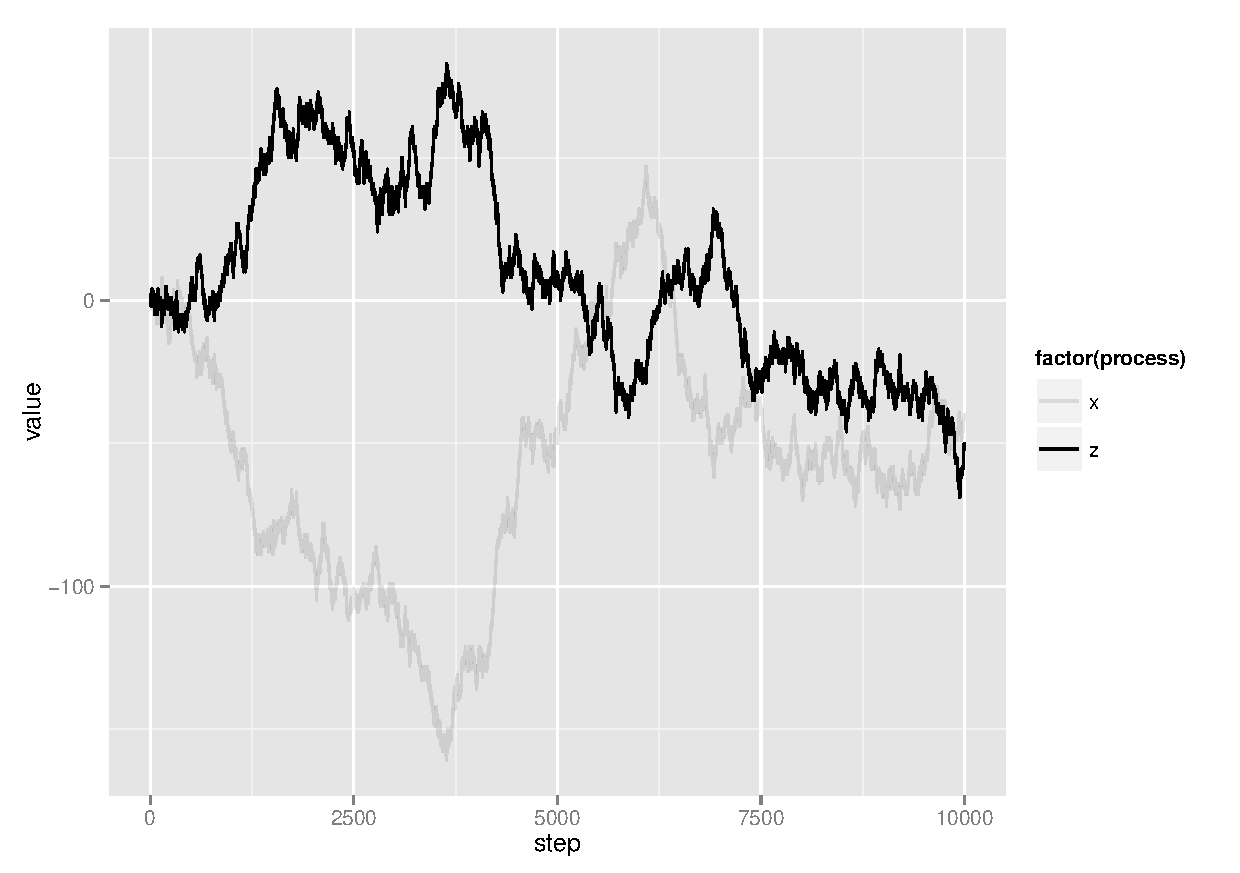
\includegraphics[width=\textwidth]{./hw5-bernoulli/bernoulli.pdf}
\caption{Plot of cumulative value of X and cumulative value of Z}
\end{figure}

\begin{lstlisting}
rho = -0.5
steps = 10000
x = vector(mode = 'numeric', length = steps)
z = vector(mode = 'numeric', length = steps)
dx = vector(mode = 'numeric', length = steps)
dz = vector(mode = 'numeric', length = steps)
random = runif(steps, 0, 1)

for(i in 2:steps) {
  if(random[i] < (1-rho) / 4) {
    x[i] = x[i-1] - 1;
    z[i] = z[i-1] + 1;
    dx[i] = -1;
    dz[i] = 1;
  } else if (random[i] < 0.5) {
    x[i] = x[i-1] + 1;
    z[i] = z[i-1] + 1;
    dx[i] = 1;
    dz[i] = 1;
  } else if (random[i] < 0.5 + (1-rho) / 4) {
    x[i] = x[i-1] + 1;
    z[i] = z[i-1] - 1;
    dx[i] = 1;
    dz[i] = -1;
  } else {
    x[i] = x[i-1] - 1;
    z[i] = z[i-1] - 1;
    dx[i] = -1;
    dz[i] = -1;
  }
}

library(ggplot2)
library(reshape)
data = cbind(x, z)
colnames(data) = c('x', 'z')
melted = melt(data, id=c('x', 'z'))
colnames(melted) = c('step', 'process', 'value')
plot = ggplot(data = melted) + geom_line(aes(x=step, y=value, colour=process))
plot

cor(dx, dz)
\end{lstlisting}

$cor(dx, dz) = -0.5003817$, fits chosen $\rho$ value pretty well.

\section{}

Let $V$ be the value of the portfolio. Since $B$ is borrowed and used to buy $S$, 

\[V = S + B - B = S\]

Then since $B$ amount of stocks are added,

\begin{align*}
dV &= \left(\frac{S+B}{S}dS -rBdt\right) \\
&= \left(S\mu + B\mu - rB\right)dt + (S+B)\sigma dZ
\end{align*}

Since we're interested in excess returns $= S\mu + B\mu - rB - Vr = S\mu + B\mu - rB - rS$, 

\[\lambda_V = \frac{S\mu + B\mu - rB - rS}{(S+B)\sigma} = \frac{\mu-r}{\sigma} = \lambda\]


\section{}

Let $i$ be index. Let $p$ be portfolio.

\[\mu_p = (1-w)\mu_f + w\mu_i\]
\[\sigma_p = w\sigma_i\]

\subsection{}

For $\sigma_p = 0.15$, $w = 0.5$. Then,

\[\mu_p = (0.5)(0.04) + 0.5(0.24) = 0.14\]

\subsection{}

You'd borrow $-0.5$ the value of the whole portfolio. ie. you'd lend as much as you invest in the index.
\end{document}
